\ifwithsols
\else
\clearpage
\fi

\subsection*{سؤال 11 امتحان 899271 سنة 2024}
\addcontentsline{toc}{subsection}{سؤال 11 امتحان 899271 سنة 2024}

\noindent
\makebox[\textwidth][c]{
\includegraphics[width=0.9\paperwidth,keepaspectratio]{ ../../../bagrut_questions/computational_models/turing_2024_899271_11.jpg }%
}%

\ifwithsols
\begin{boxSolution}[سؤال 11 امتحان 899271 سنة 2024]
\begin{enumerate}[itemsep=1.5em, label=\alph*.]

\item
\textbf{المدخل ($x=1, y=3$):}
\hfill
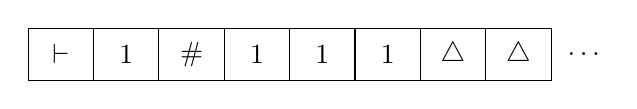
\begin{tikzpicture}[scale=0.83]
    \foreach \i/\c in {1/$\vdash$,2/1,3/\#,4/1,5/1,6/1,7/$\triangle$,8/$\triangle$} {
        \draw (\i,0) rectangle +(1,0.8);
        \node at (\i+0.5,0.4) {\c};
    }
    \node at (9.5, 0.4) {$\ldots$};
\end{tikzpicture}

\textbf{تتبع الحالات:}
{\small
\begin{align*}
q_0 \quad &\vdash \; \underline{1} \; \# \; 1 \; 1 \; 1 \; \triangle \\
q_1 \quad &\vdash \; \triangle \; \underline{\#} \; 1 \; 1 \; 1 \; \triangle \quad \text{(مسح 1 من $x$، يمين)} \\
q_2 \quad &\vdash \; \triangle \; \# \; \underline{1} \; 1 \; 1 \; \triangle \\
q_2 \quad &\vdash \; \triangle \; \# \; 1 \; \underline{1} \; 1 \; \triangle \\
q_2 \quad &\vdash \; \triangle \; \# \; 1 \; 1 \; \underline{1} \; \triangle \\
q_2 \quad &\vdash \; \triangle \; \# \; 1 \; 1 \; 1 \; \underline{\triangle} \quad \text{(تجاوز العدد الثاني)} \\
q_3 \quad &\vdash \; \triangle \; \# \; 1 \; 1 \; \underline{1} \; \triangle \quad \text{(رأى $\triangle$، رجع يسارًا)} \\
q_4 \quad &\vdash \; \triangle \; \# \; 1 \; \underline{1} \; \triangle \; \triangle \quad \text{(مسح 1 من $y$، رجع يسارًا)} \\
q_4 \quad &\vdash \; \triangle \; \# \; \underline{1} \; 1 \; \triangle \; \triangle \\
q_4 \quad &\vdash \; \triangle \; \underline{\#} \; 1 \; 1 \; \triangle \; \triangle \\
q_4 \quad &\vdash \; \underline{\triangle} \; \# \; 1 \; 1 \; \triangle \; \triangle \\
q_0 \quad &\vdash \; \triangle \; \underline{\#} \; 1 \; 1 \; \triangle \; \triangle \quad \text{(رأى $\triangle$، تقدم يمينًا لدورة جديدة)} \\
q_8 \quad &\vdash \; \triangle \; \$ \; \underline{1} \; 1 \; \triangle \; \triangle \quad \text{($q_0$ يرى $\#$: انتهى $x$، كتب $\$$، يمين)} \\
q_8 \quad &\vdash \; \triangle \; \$ \; 1 \; \underline{1} \; \triangle \; \triangle \\
q_8 \quad &\vdash \; \triangle \; \$ \; 1 \; 1 \; \underline{\triangle} \; \triangle \quad \text{(تجاوز المتبقي من $y$)} \\
q_7 \quad &\vdash \; \triangle \; \$ \; 1 \; 1 \; \$ \; \underline{\triangle} \quad \text{(كتب $\$$ النهائية وتوقف للقبول)} \checkmark
\end{align*}
}

\textbf{ماذا سينتج على الشريط في نهاية العمليّة:}
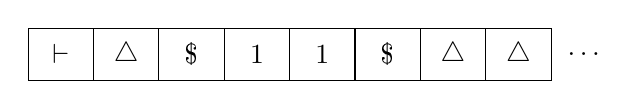
\begin{tikzpicture}[scale=0.83]
    \foreach \i/\c in {1/$\vdash$,2/$\triangle$,3/\$,4/1,5/1,6/\$,7/$\triangle$,8/$\triangle$} {
        \draw (\i,0) rectangle +(1,0.8);
        \node at (\i+0.5,0.4) {\c};
    }
    \node at (9.5, 0.4) {$\ldots$};
\end{tikzpicture}
\\
$\leftarrow$ الناتج بين الـ\$: $1\,1$ (= 2 = |1 - 3|) \checkmark \\

\end{enumerate}
\end{boxSolution}

\begin{boxSolution}
\begin{enumerate}[itemsep=1.5em, label=\alph*., resume]
\item
المدخل هو $x=2, y=1$. بعد تكرار نفس العملية، سينتج على الشريط:

\hfill
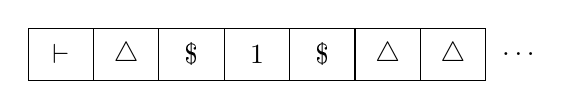
\begin{tikzpicture}[scale=0.83]
    \foreach \i/\c in {1/$\vdash$,2/$\triangle$,3/\$,4/1,5/\$,6/$\triangle$,7/$\triangle$} {
        \draw (\i,0) rectangle +(1,0.8);
        \node at (\i+0.5,0.4) {\c};
    }
    \node at (8.5, 0.4) {$\ldots$};
\end{tikzpicture}
\\
$\leftarrow$ الناتج بين الـ\$: $1$ (= 1 = |2 - 1|) \checkmark \\

\item
تقوم الآلة بحساب \textbf{القيمة المطلقة للفرق بين العددين} $f(x,y) = |x - y|$. وتقوم بوضع الناتج النهائي محصوراً بين رمزي $\$$ الأولى و$\$$ الثانية.

\item
\begin{enumerate}
    \item \textbf{العدد الأول يساوي صفرًا، والعدد الثاني أكبر من صفر (مثال $x=0, y=2$):} \\
    \textbf{حالة الآلة:} تعمل صحيحًا. \\
    \textbf{التفسير:} تبدأ الآلة بقراءة $\#$ وتحوله إلى $\$$ وتنتقل إلى الحالة $q_8$. ثم تتخطى الآحاد يميناً، وعندما تقرأ الفراغ $\triangle$ تكتب $\$$ وتتوقف بنجاح في حالة القبول $q_7$.

    {\small
    \textbf{شريط المدخلات:}
    \hfill
    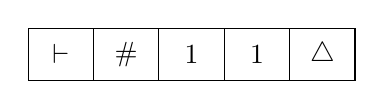
\begin{tikzpicture}[scale=0.83]
        \foreach \i/\c in {1/$\vdash$,2/\#,3/1,4/1,5/$\triangle$} {
            \draw (\i,0) rectangle +(1,0.8);
            \node at (\i+0.5,0.4) {\c};
        }
    \end{tikzpicture}

    \textbf{شريط المخرجات:}
    \hfill
    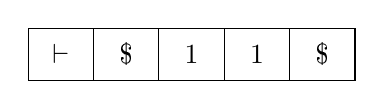
\begin{tikzpicture}[scale=0.83]
        \foreach \i/\c in {1/$\vdash$,2/\$,3/1,4/1,5/\$} {
            \draw (\i,0) rectangle +(1,0.8);
            \node at (\i+0.5,0.4) {\c};
        }
    \end{tikzpicture}
    }

    \item \textbf{العدد الثاني يساوي صفرًا، والعدد الأول أكبر من صفر (مثال $x=1, y=0$):} \\
    \textbf{حالة الآلة:} \underline{لا} تعمل صحيحًا. \\
    \textbf{التفسير:} بعد مسح الآحاد من العدد الأول (تصبح $\triangle$)، تصل الآلة لـ $\#$ وتستبدله بـ $\$$ في الحالة $q_3$ وتنتقل يساراً للحالة $q_5$. تقرأ الفراغ $\triangle$ وتستبدله بـ $1$ وتتحرك يساراً إلى الحالة $q_6$. في هذه اللحظة، سيصطدم رأس الآلة ببداية الشريط $\vdash$. نظرًا لأن الحالة $q_6$ غير معرّفة للتعامل مع الرمز $\vdash$، تتوقف الآلة قسرياً بشكل غير طبيعي (Crash) ولا تصل لحالة القبول.

    \item \textbf{العددان يساويان صفرًا ($x=0, y=0$):} \\
    \textbf{حالة الآلة:} تعمل صحيحًا. \\
    \textbf{التفسير:} تقرأ الآلة $\#$ وتحوله إلى $\$$ وتنتقل للحالة $q_8$. ثم تقرأ الفراغ $\triangle$ مباشرةً وتكتب $\$$ وتتوقف بنجاح في حالة القبول $q_7$.

    {\small
    \textbf{شريط المدخلات:}
    \hfill
    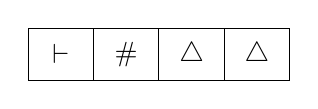
\begin{tikzpicture}[scale=0.83]
        \foreach \i/\c in {1/$\vdash$,2/\#,3/$\triangle$,4/$\triangle$} {
            \draw (\i,0) rectangle +(1,0.8);
            \node at (\i+0.5,0.4) {\c};
        }
    \end{tikzpicture}

    \textbf{شريط المخرجات:}
    \hfill
    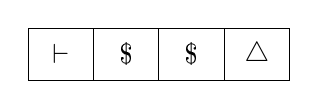
\begin{tikzpicture}[scale=0.83]
        \foreach \i/\c in {1/$\vdash$,2/\$,3/\$,4/$\triangle$} {
            \draw (\i,0) rectangle +(1,0.8);
            \node at (\i+0.5,0.4) {\c};
        }
    \end{tikzpicture}
    }
\end{enumerate}

\end{enumerate}
\end{boxSolution}

\clearpage
\fi
